% Методы задания однозначности и их отражение в архитектурах ВС

\chapter{Методы задания однозначности и их отражение в архитектурах ВС}

Одним из ключевых моментов многоуровневой организации архитектур является подход к определению однозначности операций выполняемых, компьютером. Под однозначностью в данном случае понимается четкое понимание того, какие данные какого типа поступают на вход операции и какой получается тип результата после ее выполнения. Данный вопрос непосредственно связан с представлением типов в языках программирования~\cite{types-in-prog-lang} и подходами к их использованию. Более детально эти вопросы исследуются теорией типов~\cite{types-theory}.

\section{Пример неоднозначной трактовки алгоритма}

Основные проблемы, с заданием однозначности можно рассмотреть на весьма простом примере, связанным с созданием алгоритмов на начальном этапе их изучения. Обычно в рамках этого процесса используется некоторый упрощенный язык описания алгоритмов и представляется архитектура исполнителя. Выберем в качестве представления словесное описание алгоритма с использованием следующих команд:

\begin{verbatim}
    1. Начало
    2. Конец
    3. Ввод
    4. Вывод
    5. Операция
    6. Условный переход
    7. Безусловный переход
\end{verbatim}
Данные команды вполне понятны на интуитивном уровне и позволяют разрабатывать <<программы>> для компьютера обобщенная схема которого представлена на рисунке~\ref{type-01}.
\begin{figure}[htbp]
    \centering
    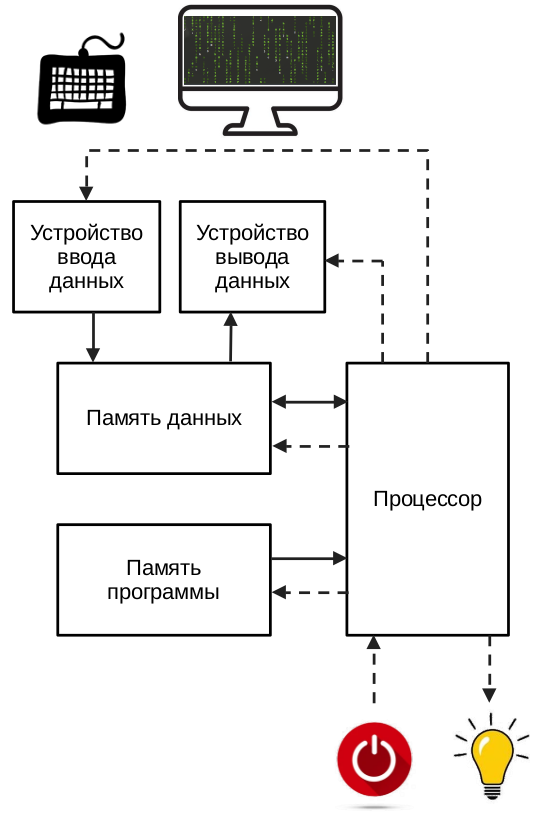
\includegraphics[width=0.4\textwidth]{img/type-01.png}
    \caption{Обобщенная архитектура простейшего исполнителя алгоритмов}
    \label{type-01}
\end{figure}
Алгоритм записывается в память программы. Данные размещаются соответственно в памяти данных. Есть некоторый ввод данных, а также вывод формируемых результатов. Операции выполняет процессор. Запуск программы осуществляется нажатием кнопки пользователем. При завершении выполнения программы загорается лампочка. В принципе на интуитивном уровне достаточно понятно как функционирует такая система.

Рассмотрим, каким образом будет выполняться на такой системе программа вычисления факториала:

\begin{ffcode}
0. Начало
1. Ввод N
2. F = 1
3. Если N < 2 На 7
4. F = F * N
5. N = N - 1
6. На 3
7. Вывод F
8. Конец
\end{ffcode}

Для имитации выполнения можно использовать ручной метод прокрутки для некоторых исходных данных. После загрузки программы наша система будет находиться в ожидании запуска (рисунок~\ref{type-02}).
\begin{figure}[htbp]
    \centering
    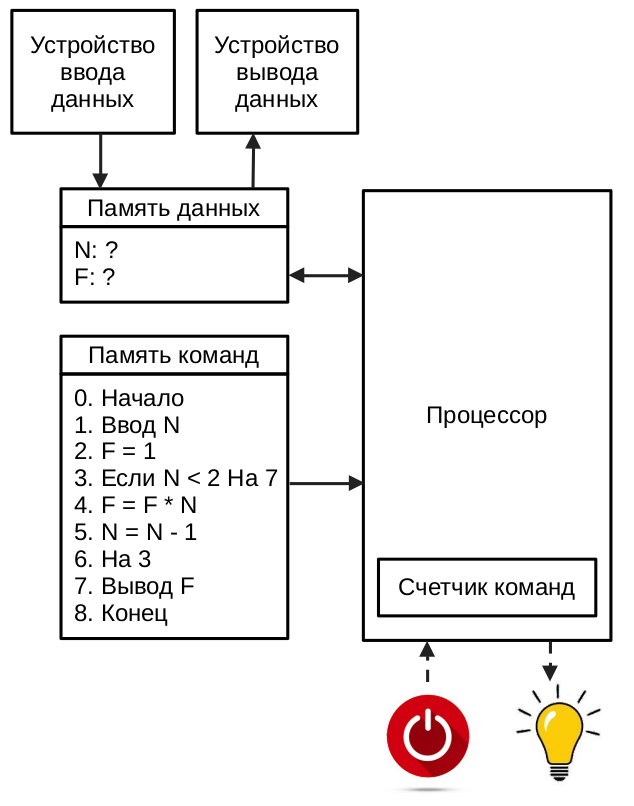
\includegraphics[width=0.4\textwidth]{img/type-02.png}
    \caption{Обобщенная архитектура простейшего исполнителя алгоритмов}
    \label{type-02}
\end{figure}
После нажатия на кнопку запуска программы система ищет начальную команду, устанавливая счетчик команд в нулевое значение (рисунок~\ref{type-03}). Затем осуществляется переход в автоматический режим с переключение на следующую команду счетчика команд.
\begin{figure}[htbp]
    \centering
    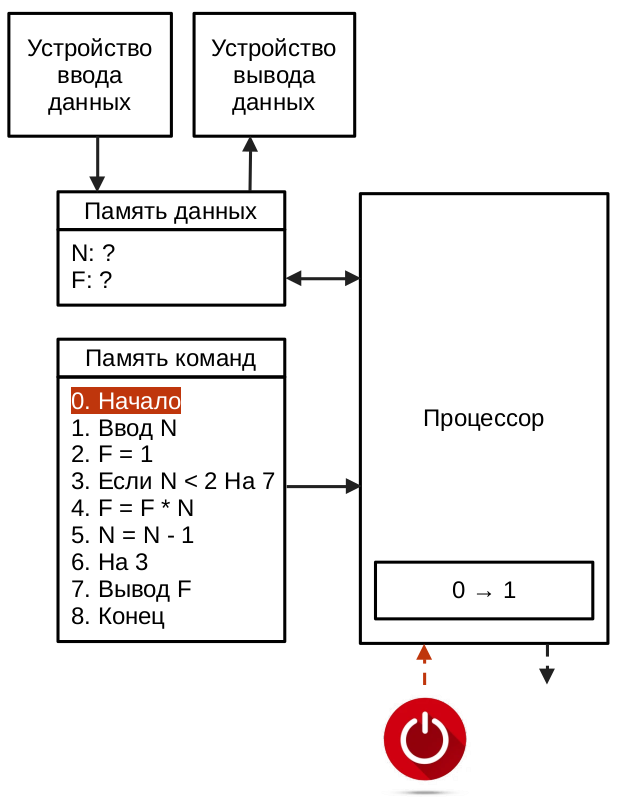
\includegraphics[width=0.4\textwidth]{img/type-03.png}
    \caption{Обобщенная архитектура простейшего исполнителя алгоритмов}
    \label{type-03}
\end{figure}
Выполнение команды ввода в команде 1 позволяет получить значение операнда N (рисунок~\ref{type-04}).
\begin{figure}[htbp]
    \centering
    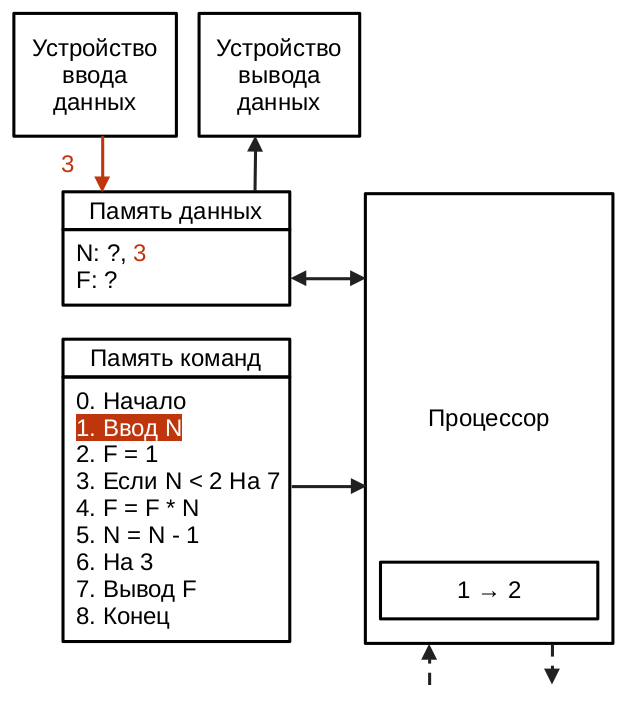
\includegraphics[width=0.4\textwidth]{img/type-04.png}
    \caption{Обобщенная архитектура простейшего исполнителя алгоритмов}
    \label{type-04}
\end{figure}

\begin{figure}[htbp]
    \centering
    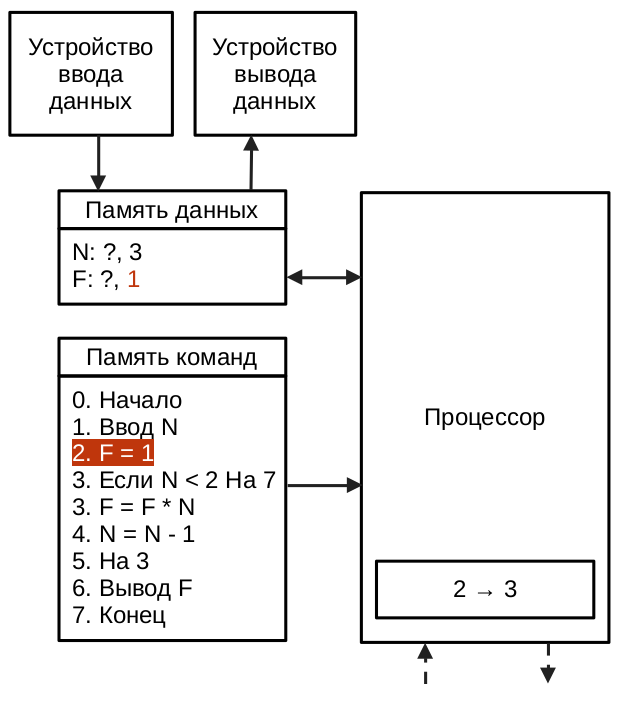
\includegraphics[width=0.4\textwidth]{img/type-05.png}
    \caption{Обобщенная архитектура простейшего исполнителя алгоритмов}
    \label{type-05}
\end{figure}
Следующая команда присваивает переменной F значение, равное  1 (рисунок~\ref{type-05})

Дальнейшие вычисления выполняются в автоматическом режиме до выполнения команды завершения программы (рисунок~\ref{type-13}).
\begin{figure}[htbp]
    \centering
    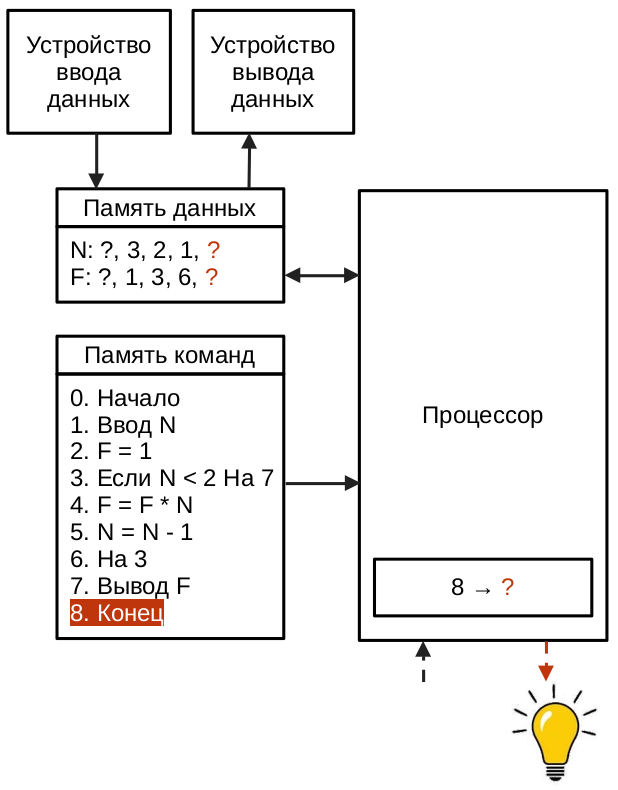
\includegraphics[width=0.4\textwidth]{img/type-13.png}
    \caption{Обобщенная архитектура простейшего исполнителя алгоритмов}
    \label{type-13}
\end{figure}

\textbf{примечание.}
\textit{Пока описано как есть. Возможно стоит описать более подробно все шаги и подставить все необходимые рисунки.}

Глядя на приведенный алгоритм и понимая его только на интуитивном уровне, человек может получить конечный результат, опираясь на свой опыт и знания даже в условиях неоднозначного представления информации. В частности, его мало волнуют следующие вопросы:
\begin{itemize}
    \item Можно ли использовать действительные числа, символы, строки?
	\item Как воспринимается ввод данных?
	\item Как отображаются данные?
	\item На какие устройства ввода-вывода можно использовать?
	\item Какова семантика каждой выполняемой операции?
	\item Какой тип памяти данных у N и F?
\end{itemize}
Возникает также вопрос: а может ли реальный компьютер выполнить данный алгоритм без наличия представленной выше информации?

Реализуем на языке программирования С аналогичную программу для компьютера и посмотрим, что изменилось.

\begin{ffcode}
#include <stdio.h>

static int n;
static int f = 1;

int main() {
  // Во время выполнения:
  printf("n? ");           // calc(char*)
  scanf("%d", &n);         // calc(char*); if(%d)-> use n as int
loop:
  // Во время компиляции:
  if(n < 2) goto end;      // <(int, int) -> bool
  f *= n;                  // *(int, int) -> int; =(int) -> int
  n--;                     // --(int) -> int
  goto loop;
end:
  // Во время выполнения:
  printf("n! = %d\n", f);  // calc(char*); if(%d)-> use n as int
}
\end{ffcode}
Мы видим, что появились описания типов данных, которые обеспечивают поддержку однозначности при выполнении операций. Любая выполняемая операция имеет полную информацию о своих аргументах, что позволяет однозначно сформировать тип и значения результата. Подобный контроль данных позволяет компьютеру не <<задумываться>> о том, с каким данными он работает. За него обо всем позаботился программист, предоставив всю необходимую информацию для компилятора.

Однако на самом деле не все так безоблачно, так как не всю информацию можно четко определить во время компиляции. Это касается вводимых в программу данных. Они вводятся в символьном виде и преобразуются во внутреннее представление на этапе вычислений. Следовательно корректность ввода и преобразования из вне во внутрь осуществляются компьютером и при некорректном вводе данных могут привести к неправильным результатам. Это говорит о том, что динамические трансформации и их контроль необходимы и в случае четкого контроля выполняемых действий. Данную программу легко сделать неправильной только изменением форматов для вводимых и (или) выводимых данных:

\begin{ffcode}
#include <stdio.h>

static int n;
static int f = 1;

int main() {
  // Во время выполнения:
  printf("n? ");            // calc(char*)
  scanf("%c", &n);          // calc(char*); if(%c)-> use n as char
loop:
  // Во время компиляции:
  if(n < 2) goto end;       // <(int, int) -> bool
  f *= n;                   // *(int, int) -> int; =(int) -> int
  n--;                      // --(int) -> int
  goto loop;
end:
  // Во время выполнения:
  printf("n! = %s\n", f);  // calc(char*); if(%s)-> use n as char*
}
\end{ffcode}

\section{Способы задания однозначности}

\textbf{Однозначность} определяет четкие правила выполнения операций реальными и виртуальными вычислительными системами, позволяя избегать или обходить ошибки программирования.

Различные методы задания однозначности операций позволяют контролировать корректность программы с разной степенью и на различных стадиях обработки 

Существуют различные виды однозначности, что напрямую связано с использованием типов в языках программирования:
\begin{enumerate}
    \item операционная однозначность (бестиповые системы);
    \item динамическая однозначность (системы с динамической типизацией);
    \item статическая однозначность (системы со статической типизацией).
\end{enumerate}
Также можно отметить, что в языках программирования обычно используются все подходы независимо от того, как позиционируется сам язык. Это отражается и на многоуровневую организацию архитектур ВС.

\subsection{Операционная однозначность}

Операционная однозначность, определяется через операции того или иного языка программирования, определяющего архитектуру реальной или виртуальной ВС. Она формируется за счет четкого определения что и с какими типами данных делает каждая операция. Сами данные при этом не несут никакой дополнительной информации о своем типе и рассматриваются в виде совокупности байт (бит), размещенных в памяти. Доступ к обезличенным данным осуществляется по адресам, задаваемым в операциях. Для таких архитектур характерны бестиповые языки.

Примеры подобных архитектур:
\begin{itemize}
    \item современные (традиционные) архитектуры уровня системы команд и их языки ассемблера;
    \item объектно-ориентированный язык программирования Eolang (и архитектура его виртуальной машины);
    \item частичная поддержка в языках системного программирования.
\end{itemize}

Реализаци бестипового программирования обычно осуществляется на уровне системы команд, характерном практически для всех существующих архитектур ВС. Каждая команда определяет операцию над обезличенными данным с учетом специфики той или иной архитектуры и реализации языка Ассемблера. Например, низкоуровневая программа, написанная с использованием Gnu Assembler и библиотеки \code{libc} будет выглядеть следующим образом:

\begin{ffcode}
# asm-fact.s
    .intel_syntax noprefix
# Константные данные
    .section  .rodata
question:
    .string "n? "
    .equ    questionLength, .-question-1
formatIn:
    .string "%d"
    .equ    formatInLength, .-formatIn-1
formatOut:
    .string "n! = %d\n"
    .equ    formatOutLength, .-formatOut-1

# Статические переменные
    .data
n:  .long   0

# Текст программы
    .text
    .globl  main
main:
    push    rbp                     # пролог
    mov     rbp, rsp

    # Ввод начального значения n
    lea     rdi, question[rip]      # адрес формата подсказки
    mov     eax, 0                  # не действительные числа
    call    printf@plt              # печать подсказки

    lea     rdi, formatIn[rip]      # адрес формата числа
    lea     rsi, n[rip]
    mov     eax, 0                  # не действительные числа
    call    scanf@plt               # ввод целого

    # Вычисление факториала
    mov     eax, 1                  # начальная установка f
    mov     ebx, n[rip]             # перенос n в регистр
loop:
    cmp     ebx, 2                  # проверка на завершение
    jl      end                     # выход по меньше
    mul     ebx                     # f *= n
    dec     ebx                     # --n;
    jmp     loop
end:

    # Вывод результата вычислений
    lea     rdi, formatOut[rip]     # адрес формата результата
    mov     rsi, rax                # значение результата
    mov     eax, 0                  # не действительные числа
    call    printf@plt              # печать результата

    mov     eax, 0                  # return 0
    pop     rbp                     # эпилог
    ret
\end{ffcode}

Использование бестипового программирования не обязательно рассматривать на языках уровня системы команд. Необходимость эффективной манипуляции с компьютерной памятью ведет к тому, что в языках системного программирования используются конструкции, позволяющие легко писать бестиповой код. Поэтому программу, осуществляющую вычисление факториала можно представить следующим образом:

\begin{ffcode}
#include <stdio.h>

static char memory[2*sizeof(int)];     // Память для n и f
static void* n = memory;               // Адрес на область для n
static void* f = memory + sizeof(int); // Адрес на область для f

int main() {
    *((int*)f) = 1;
    printf("n? ");
    scanf("%d", n);
    printf("n = %d\n", *((int*)n));
    printf("f = %d\n", *((int*)f));
loop:
    if(*((int*)n) < 2) goto end;
    *((int*)f) *= *((int*)n);
    (*(int*)n)--;
    goto loop;
end:
    printf("n! = %d\n", (*(int*)f));
}
\end{ffcode}
Отображение на компьютерную память в данном случае осуществляется с использованием символьного массива, обеспечивающего резервирование в ней соответствующего числа байт. Адреса в этомй памяти для \code{n} и \code{f} фиксируются через соответствующие указатели. Для того, чтобы операции языка C имели информацию об обрабатываемых ими типах данных, необходимо явным образом осуществить их приведение к нужном типу. Это приведение возлагается на программиста, что может вести к ошибкам при написании больших программ в бестиповом стиле.

\subsection{Динамическая однозначность}

Динамическая однозначность операций формируется за счет того, что с каждым значением, формируемым в программе сопоставляется его тип. Любая операция над данным может проверить этот тип и выбрать в соответствии с этим нужные вычисления. То есть, одна и та же операция может обрабатывать различные типы данных. При этом идентификация типа осуществляется во время выполнения программы. Одни и те же переменные могут хранить данные различного типа. В любой момент программа может проверить тип переменной. Данный подход широко используется в языках программирования, ориентированных на интерпретацию.

Примеры подобных архитектур:
\begin{itemize}
    \item Языки сценариев: Python, JavaScript, Lua и~др.;
    \item Языки функционального программирования: Lisp и~др.
\end{itemize}
Следует отметить, что в настоящее время практически отсутствую аппаратные решения, ориентированные на поддержку динамической однозначности. Хотя одно время (до эпохи сверхбольших интегральных схем) существовали несколько проектов~\cite{modern-arch}. В качестве примера можно отметить процессор фирмы Intel iAPX~432~\cite{i432-1,i432-2}.


\subsection{Статическая однозначность}

\textbf{Статическая однозначность} операций формируется за счет того, что с каждым значением в программе сопоставляется его тип. Этот тип задается при описании переменных и может быть проверен во время компиляции. Для всех временных и промежуточных значений тип может быть также выведен во время компиляции. Поэтому его не имеет смысла проверять во время выполнения. Одна и та же операция может быть задана с разными типами, но все вопросы по ее конкретному выполнению решаются во время компиляции (статический полиморфизм). С каждой переменной сопоставляется только один тип.Допускает эффективную трансформацию в бестиповые архитектуры уровня системы команд. Используется в языках компилируемого типа.

Примеры подобных архитектур:
\begin{itemize}
    \item Императивные языки программирования:C, C++, Pascal, Oberon family, Java, C\#, Rust, Go и~др;
    \item Языки функционального программирования: ML, Haskell и~др.
\end{itemize}
Из-за возможностей эффективной компиляции статически типизируемых программ в бестиповые практически отсутствует необходимость в разработке аппаратных решений для таких архитектур. Однако понимание, каким образом в ходе компиляции происходят трансформации из одной архитектуры в другую необходимы в связи с распространенностью языков со статической типизацией, обеспечивающих при программировании наиболее высокую надежность ПО за счет тотального контроля на этапе компиляции.

Завершая данный раздел следует отметить, что в разных частях больших программ мог могут применяться различные решения, что определяется как особенностью решаемой задачи, так и спецификой используемого языка программирования. В частности, при обработке данных альтернативных типов приходится моделировать их динамическую проверку за счет использования специальных тегов. Для передачи произвольных данных в функции языки C и C++ предоставляют указатель на \code{void}, который обеспечивает поддержку бестипового программирования.